\begin{frame}{Featureless Insulators}
\vskip-1.5cm
\begin{columns}[T]
    \begin{column}[T]{.6\textwidth}
        \begin{block}{Definition of `Featureless Insulator'}
            \vskip-1em
            \begin{itemize}
                % 0 T G.S. of quantum Hamiltonians
            \item Gapped 
                %Energy gap to excitations
            \item Symmetric 
                %G.S. Wavefunc preserves all symmetries of the Hamiltonian, no local order parameter - no spontaneous symmetry breaking
            \item No topological order %exotic statistics
                %insulator ->assume that we have a U(1) symmetry by which to define charge
            \item Integer charge per unit cell
                %unit cell -> also assuming discrete translational symmetry
            \item Unique ground state with P.B.C.
                %This can be made into the defining property, all of these others follow from this.
                % Response to change in B.C. can be, with some work, a way to distinguish gapped phases of matter
            \end{itemize}
        \end{block}
    \vskip-0.5cm    
    Examples:
    \end{column}
    \begin{column}[T]{.4\textwidth}
    \begin{figure}[h]
            \centering
            \scalebox{0.7}{
            %
% x=3*(minimum size)/2
% y=\sqrt{3/4}*(minimum size)/2
%

%http://tex.stackexchange.com/questions/6019/drawing-hexagons
\begin{tikzpicture}[x=7.5mm,y=4.33mm]
  % some styles
  \tikzset{
    box/.style={
      regular polygon,
      regular polygon sides=6,
      minimum size=10mm,
      inner sep=0mm,
      outer sep=0mm,
      rotate=0,
    draw
    }
  }
 \tikzset{boson/.style={circle=1pt,draw=black!100,fill=orange!100,inner sep=2pt}}

\foreach \i in {0,...,2} 
    \foreach \j in {0,...,3} {
            \node[box] at (2*\i,2*\j) {};
        }
\foreach \i in {0,...,1} 
    \foreach \j in {0,...,2} {
   	   \node[box] at (2*\i+1,2*\j+1) {};   
        }
\foreach \i in {0,...,2} 
    \foreach \j in {0,...,3} {
            \node[boson] at (2*\i-0.6,2*\j) {};
            \node[boson] at (2*\i+0.6,2*\j) {};
            \node[boson] at (2*\i-0.4,2*\j-1) {};
            \node[boson] at (2*\i-0.4,2*\j+1) {};
             \node[boson] at (2*\i+0.4,2*\j+1) {};
              \node[boson] at (2*\i+0.4,2*\j-1) {};
        }
%\foreach \i in {0,...,1} 
  %  \foreach \j in {0,...,2} {
%	\node[boson] at (2*\i+1-0.6,2*\j+1) {}; 
%	\node[boson] at (2*\i+1+0.6,2*\j+1) {};   
   %   }
      
\end{tikzpicture}

            }
            %Atomic insulator
            \caption{\begin{tabular}[t]{l}
                     Bosonic Mott insulator \\
                     with integer filling \end{tabular}}
    \end{figure}
    \end{column}
\end{columns}

\begin{columns}[T]
    \begin{column}[T]{.4\textwidth}
        \vskip-0.5cm
        \begin{figure}[h]
            \centering
            \scalebox{0.6}{
             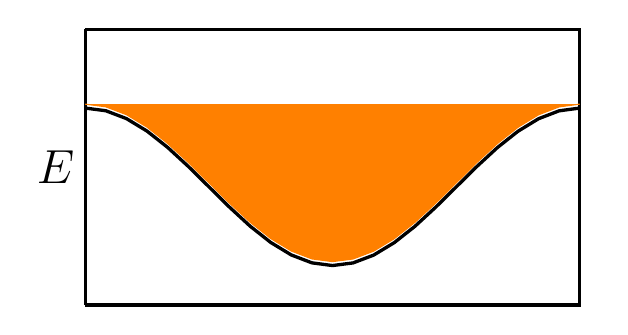
\begin{tikzpicture}[domain=0:6.28]
      \draw[very thick] (0, -2.5) -- (0,1) node[left, midway] {\LARGE $E$} ;
      \draw[very thick] (0, 1)-- (6.28,1) -- (6.28, -2.5) -- (0, -2.5);
      \draw[color=black, very thick] plot (\x,{-1+cos(\x r)}) node[right] {};
      \draw[color=orange, fill] plot (\x,{-0.95+cos(\x r)}) {};
  \end{tikzpicture}
  
            }
        \caption{Band Insulator}
        \end{figure}
    \end{column}
    \begin{column}[T]{.6\textwidth}
        \begin{figure}[h]
            \scalebox{1.4}{
            \tikzset{eli/.style={ellipse, rotate=0, draw=black, fill=gray!20}}
\tikzset{button/.style={
% First preaction: Fuzzy shadow
preaction={fill=black,path fading=circle with fuzzy edge 20 percent,
opacity=.5,transform canvas={xshift=1mm,yshift=-1mm}},
% Second preaction: Background pattern
preaction={pattern=#1,
path fading=circle with fuzzy edge 15 percent},
% Third preaction: Make background shiny
preaction={top color=white,
bottom color=black!50,
shading angle=45,
path fading=circle with fuzzy edge 15 percent,
opacity=0.2},
% Fourth preaction: Make edge especially shiny
preaction={path fading=fuzzy ring 15 percent,
top color=black!5,
bottom color=black!80,
shading angle=45},
inner sep=2ex
},
button/.default=horizontal lines light blue,
circle}
\usetikzlibrary{backgrounds}
\pgfdeclarelayer{background}
\pgfsetlayers{background,main}
\begin{tikzpicture}
\begin{scope}[on background layer]
\node[eli] at (0,0) {$\,\,\,$};
\node[eli] at (0.7,0) {$\,\,\,$};
\node[eli] at (1.4,0) {$\,\, \,$};
\node[eli] at (2.1,0) {$\,\, \,$};
\end{scope}

\node[inv] (s0) at (-0.1, -0.1){};
\node[inv] (t0) at (-0.1,  0.1){};
\path[->, thick, orange] (s0.center) edge (t0.center);

\node[inv] (s1) at (0.1, -0.1){};
\node[inv] (t1) at (0.1,  0.1){};
\path[->, thick, orange] (s1.center) edge (t1.center);

\node[inv] (s2) at (0.6, -0.1){};
\node[inv] (t2) at (0.6,  0.1){};
\path[<-, thick, orange] (s2.center) edge (t2.center);

\node[inv] (s3) at (0.8, -0.1){};
\node[inv] (t3) at (0.8,  0.1){};
\path[->, thick, orange] (s3.center) edge (t3.center);

\node[inv] (s4) at (1.3, -0.1){};
\node[inv] (t4) at (1.3,  0.1){};
\path[<-, thick, orange] (s4.center) edge (t4.center);

\node[inv] (s5) at (1.5, -0.1){};
\node[inv] (t5) at (1.5,  0.1){};
\path[->, thick, orange] (s5.center) edge (t5.center);

 \node[inv] (s6) at (2.0, -0.1){};
 \node[inv] (t6) at (2.0,  0.1){};
\path[<-, thick, orange] (s6.center) edge (t6.center);

\node[inv] (s7) at (2.2, -0.1){};
\node[inv] (t7) at (2.2,  0.1){};
\path[<-, thick, orange] (s7.center) edge (t7.center);

\foreach \i in {0, 1, 2, 3}{
\node[inv] (u\i) at (0.7*\i-0.1, 0){};
\node[inv] (v\i) at (0.7*\i+0.1, 0){};
}
\node[inv] (u4) at (0.7*4-0.2, 0){};
\node[inv] (vm1) at (-0.5, 0){};

\draw[color=black] (vm1.center)  -- (u0.center);
\draw[ color=black] (v0.center)  -- (u1.center);
\draw[ color=black] (v1.center)  -- (u2.center);
\draw[ color=black] (v2.center)  -- (u3.center);
\draw[color=black] (v3.center)  -- (u4.center);

\node[] at (-0.7, 0){...};
\node[] at (2.8, 0){...};

\end{tikzpicture}
            }
            \caption{Heisenberg AF Spin-1 chain}
        \end{figure}
    \end{column}
\end{columns}
\end{frame}